\documentclass[11pt]{article}
%Gummi|065|=)
\title{\textbf{
caracteristicas de los convertidores de potencia}}
\author{Guzman Vazquez Jaime Alan Yamil}
\date{17-sep-19}
\usepackage{graphicx}
\begin{document}

\maketitle

\section{introduccion.}

En este documento abundaremos sobre los distintos convertidores de potencia, asi como sus diferentes funciones y aplicaciones, sera a manera de sintesis, se exploraran los convertidores como los son:CA-CD,CD-CA,CA-CA,CD-CD.

\maketitle
\section{CA-CD.}
un convertidor de corriente alterna a corriente directa parte de un rectificador de onda completa, su carga puede ser puramente resistiva, al agregarle a este rectificador un capacitor en paralelo el convertidor se comporta como un filtro ya que produce un voltaje en la salida basicamente continuo,
el convertidor nos proporciona una base de señal de salida basicamente rectificada\\
A mi comprension los convertidores de potencia  tienen un funcionamiento basico que por medio del rectificador o de la rectificacion y con ayuda de un capacitor hacen que una señal con variaciones grandes, con voltajes positivos y negativos se forme una señal mas y mas estable por asi decirlo y que su frecuencia sea menor hasta el punto que pueda ser usado como corriente directa , porque aunque esta siga teniendo variaciones , se considera que son muy pequeñas para que afecten de manera importante.\\
Este tipo de configuracion es la mas utilizada ya que transforma la señal que viene por defecto a señal de corriente continua, en donde la mayoria de aparatos y dispositivos trabajan , en casas, edificios, incluso en fabricas se utiliza esta configuracion mucho debido a su vertzatilidad y usos ademas de ser estandar en la industria .\\
a continuacion veremos una imagen del esquematico de un convertidor AC-DC.\\
\begin{figure}[htp]
\centering
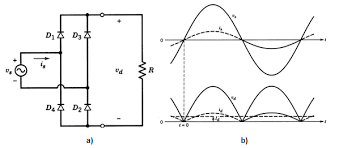
\includegraphics[scale=0.50]{/home/emile/Escritorio/ca-cd.png}
\caption{esquematico AC-DC}
\label{esquematico AC-DC}
\end{figure}
 
\title
\section{CD-CA}.
los convertidores de corriente directa a alterna son comunmente utilzados como drivers de motores y como fuentes de corriente alterna ininterumpidas y tienen como abjetivo producir señales de corriente alterna de forma sinusoidal, cuya magnitud y frecuencia pueden ser manipuladas.\\\\
Exisen diferentes tipos de convertidores inversores de los cuales existen de una sola pierna, convertidor de puente de media y connvertidor de onda completa \\\\
En las topologias antes mencionadas existe lo que se conoce como conmutacion imperfecta que es la mayor contribuyente a este tipo de convertidor ya que genera una perdida de potencia,\\
estos dispositivos absorve potencia cuando su interruptores se encienden o apagan, si la transicion se produce cuando tanto la corriete y el voltaje so diferntes a cero. si se aumenta la frecuencia de conmmutacion, estas interupciones de potencia aumentan en frecuencia y por lo tanto la perdida media de los interruptores aumenta.\\\\
Este tipo  de configuracion se interpreta como que al momento de encender y apagar los interruptores se produce una interrupcion, lo que hace que se acumule en cierta forma cuando se hace de forma repetitiva y de gran frecuencia , esto es lo que forma por asi decirlo la forma sinusoidal, las aplicaciones que yo encontraria en esta configuracion es cuando necesitas una onda sinusoidal pero con una onda y señal especifica, sin variaciones , ni nada por el estilo, ya que sacar esa señal  desde la corriente que llega desde el transformador o la corriente comun que llega a todos los lugares esta repleta de variaciones y cuestiones que pueden arriesgar tus dispositivos o las mediciones correspondientes.\\
A continuacion se mostraran imagenes sobre diagramas de estos convertidores;\\
\begin{figure}[htp]
\centering
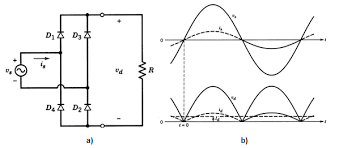
\includegraphics[scale=0.50]{/home/emile/Escritorio/dc-ac.png}
\caption{esquematico 1 configuracion DC.AC}
\label{esquematico 1 configuracion DC-AC}
\end{figure}
\begin{figure}[htp]
\centering
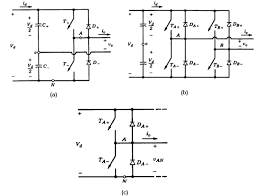
\includegraphics[scale=0.50]{/home/emile/Escritorio/dc-ca1.png}
\caption{esquematico 2 configuracion DC.AC}
\label{esquematico 2 configuracion DC-AC}
\end{figure}

Added for your viewing convenience is a continuous preview mode for the PDF. This mode is enabled by default, but can also be disabled through the \emph{(View $\rightarrow$ Page layout in preview)} menu. Complementary to this feature is SyncTeX integration, which allows you to synchronize the position in your editor with the PDF preview. 

\section{Feedback}
We hope you will enjoy using this release as much as we enjoyed creating it. If you have comments, suggestions or wish to report an issue you are experiencing - contact us at: \emph{https://github.com/alexandervdm/gummi}.

\section{One more thing}
If you are wondering where your old default text is; it has been stored as a template. The template menu can be used to access and restore it. 

\end{document}
